% dark matter, v1.0

\chapter{The Case for Dark Matter}

\paragraph{Abstract} In this chapter we outline the evidence supporting the existence of dark matter, provide a brief discussion of possible models describing what dark matter might be, and review detection schemes.

\section{Evidence for Dark Matter}

For most of the last century evidence for the existence of dark matter has been gathering from various sources. In the 1920s Edwin Hubble showed conclusively that the universe was much more than just our Milky Way galaxy~\cite{Hubble:1929}. Very soon it became clear that the universe was a very large place and that we understood very little about it.

\subsection{Galactic Rotation curves}

In the early 17th century Johannes Kepler published his three laws of planetary motion~\cite{Kepler}. Kepler's Third law is easily derived with the help of Newtonian gravitation and centripetal motion for the case of a circular orbit:
\begin{equation} \label{eq:rotation_curve}
\frac{a^3}{T^2} = \frac{GM}{4\pi^2} \Longrightarrow v(r) = \sqrt{\frac{GM}{r}}
\end{equation}
where $a$ is the orbital semimajor axis ($r$ if circular), $T$ the orbital period, $G$ the gravitational constant, $M$ the mass of the central body, and $v$ the orbital speed (assuming a circular orbit). If we assume the mass distribution is a function purely of radius, we can define
\begin{equation} \label{eq:mass_distribution}
M(r) = \int_0^r \dd^3r^{\prime}\, \rho (r^{\prime}) = 4\pi\,\int_0^r \dd r^{\prime}\, r^{\prime 2} \rho(r^{\prime})
\end{equation}
and generalize the expression Kepler found to give us a relationship relating the expected orbital velocity of an object in a galaxy as a function of its distance from the galactic core.

Armed with equations~\eqref{eq:mass_distribution} and~\eqref{eq:rotation_curve}, we can calculate $M(r)$ by observing a galaxy with telescopes and assuming some stellar mass distribution, and then make some prediction for $v(r)$. Using Doppler-shifted lines of stars or dwarf galaxies, the orbital velocities can be measured and compared to the prediction from the mass distribution, as seen in figure~\ref{fig:rotation_curve} from the Triangulum galaxy (M33)~\cite{Corbelli:1999af}.

\begin{figure}[htb]
\centering
    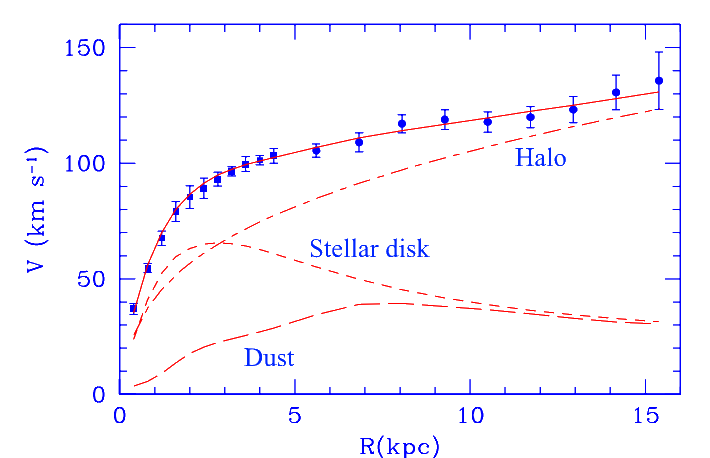
\includegraphics[width=0.8\textwidth]{figures/dm/m33_rotation}
    \caption{Rotation curve of M33, from~\cite{Corbelli:1999af}. The measured rotation speeds cannot be explained by the observed distribution of stars and dust and require the addition of a hidden source of mass to reproduce the observations.}\label{fig:rotation_curve}
\end{figure}

If we assume that stars, gas, dust, and other objects visible with telescopes are the dominant components of the galaxy, then at large distances from the galactic center it will increasingly appear like a point mass, giving the familiar relationship $v(r) \sim r^{-1/2}$ that is Kepler's third law. In the bulge in the center of the galaxy, we see the speed increases roughly linearly with the radius, while at large radii the velocity is approximately constant or increasingly slowly. However, the mass required to produce this effect is not evident in any telescope. Additionally, the stars near the edge of the galaxy are well above the predicted escape velocity $v_{\n{esc}} = \sqrt{2}v_{\n{circ}}$. Galaxies are stable over astronomical periods of time, so they cannot be filled with objects exceding the escape velocity. From this, we can propose some mass distribution that has a negligible contribution in the inner parts of the galaxy but becomes dominant at large radii~\cite{Navarro:1995iw,Graham:2005xx}.

\subsection{Gravitational lensing}

One prediction of Einstein's Theory of General Relativity is that any concentration of matter and energy will act as a lens for passing photons by distorting spacetime~\cite{Einstein:1936}. The amount and manner of lensing observed indicates the amount of matter present.

\subsubsection{Strong lensing}

Strong lensing is when images of background galaxies experience significant distortion or form multiple images by foreground objects. A good example is Einstein's Cross (QSO 2237+0305)~\cite{einstein_cross}, as shown in Figure~\ref{fig:einstein_cross}, where a distant quasar forms four images around a foreground galaxy.

\begin{figure}[htb]
    \centering
    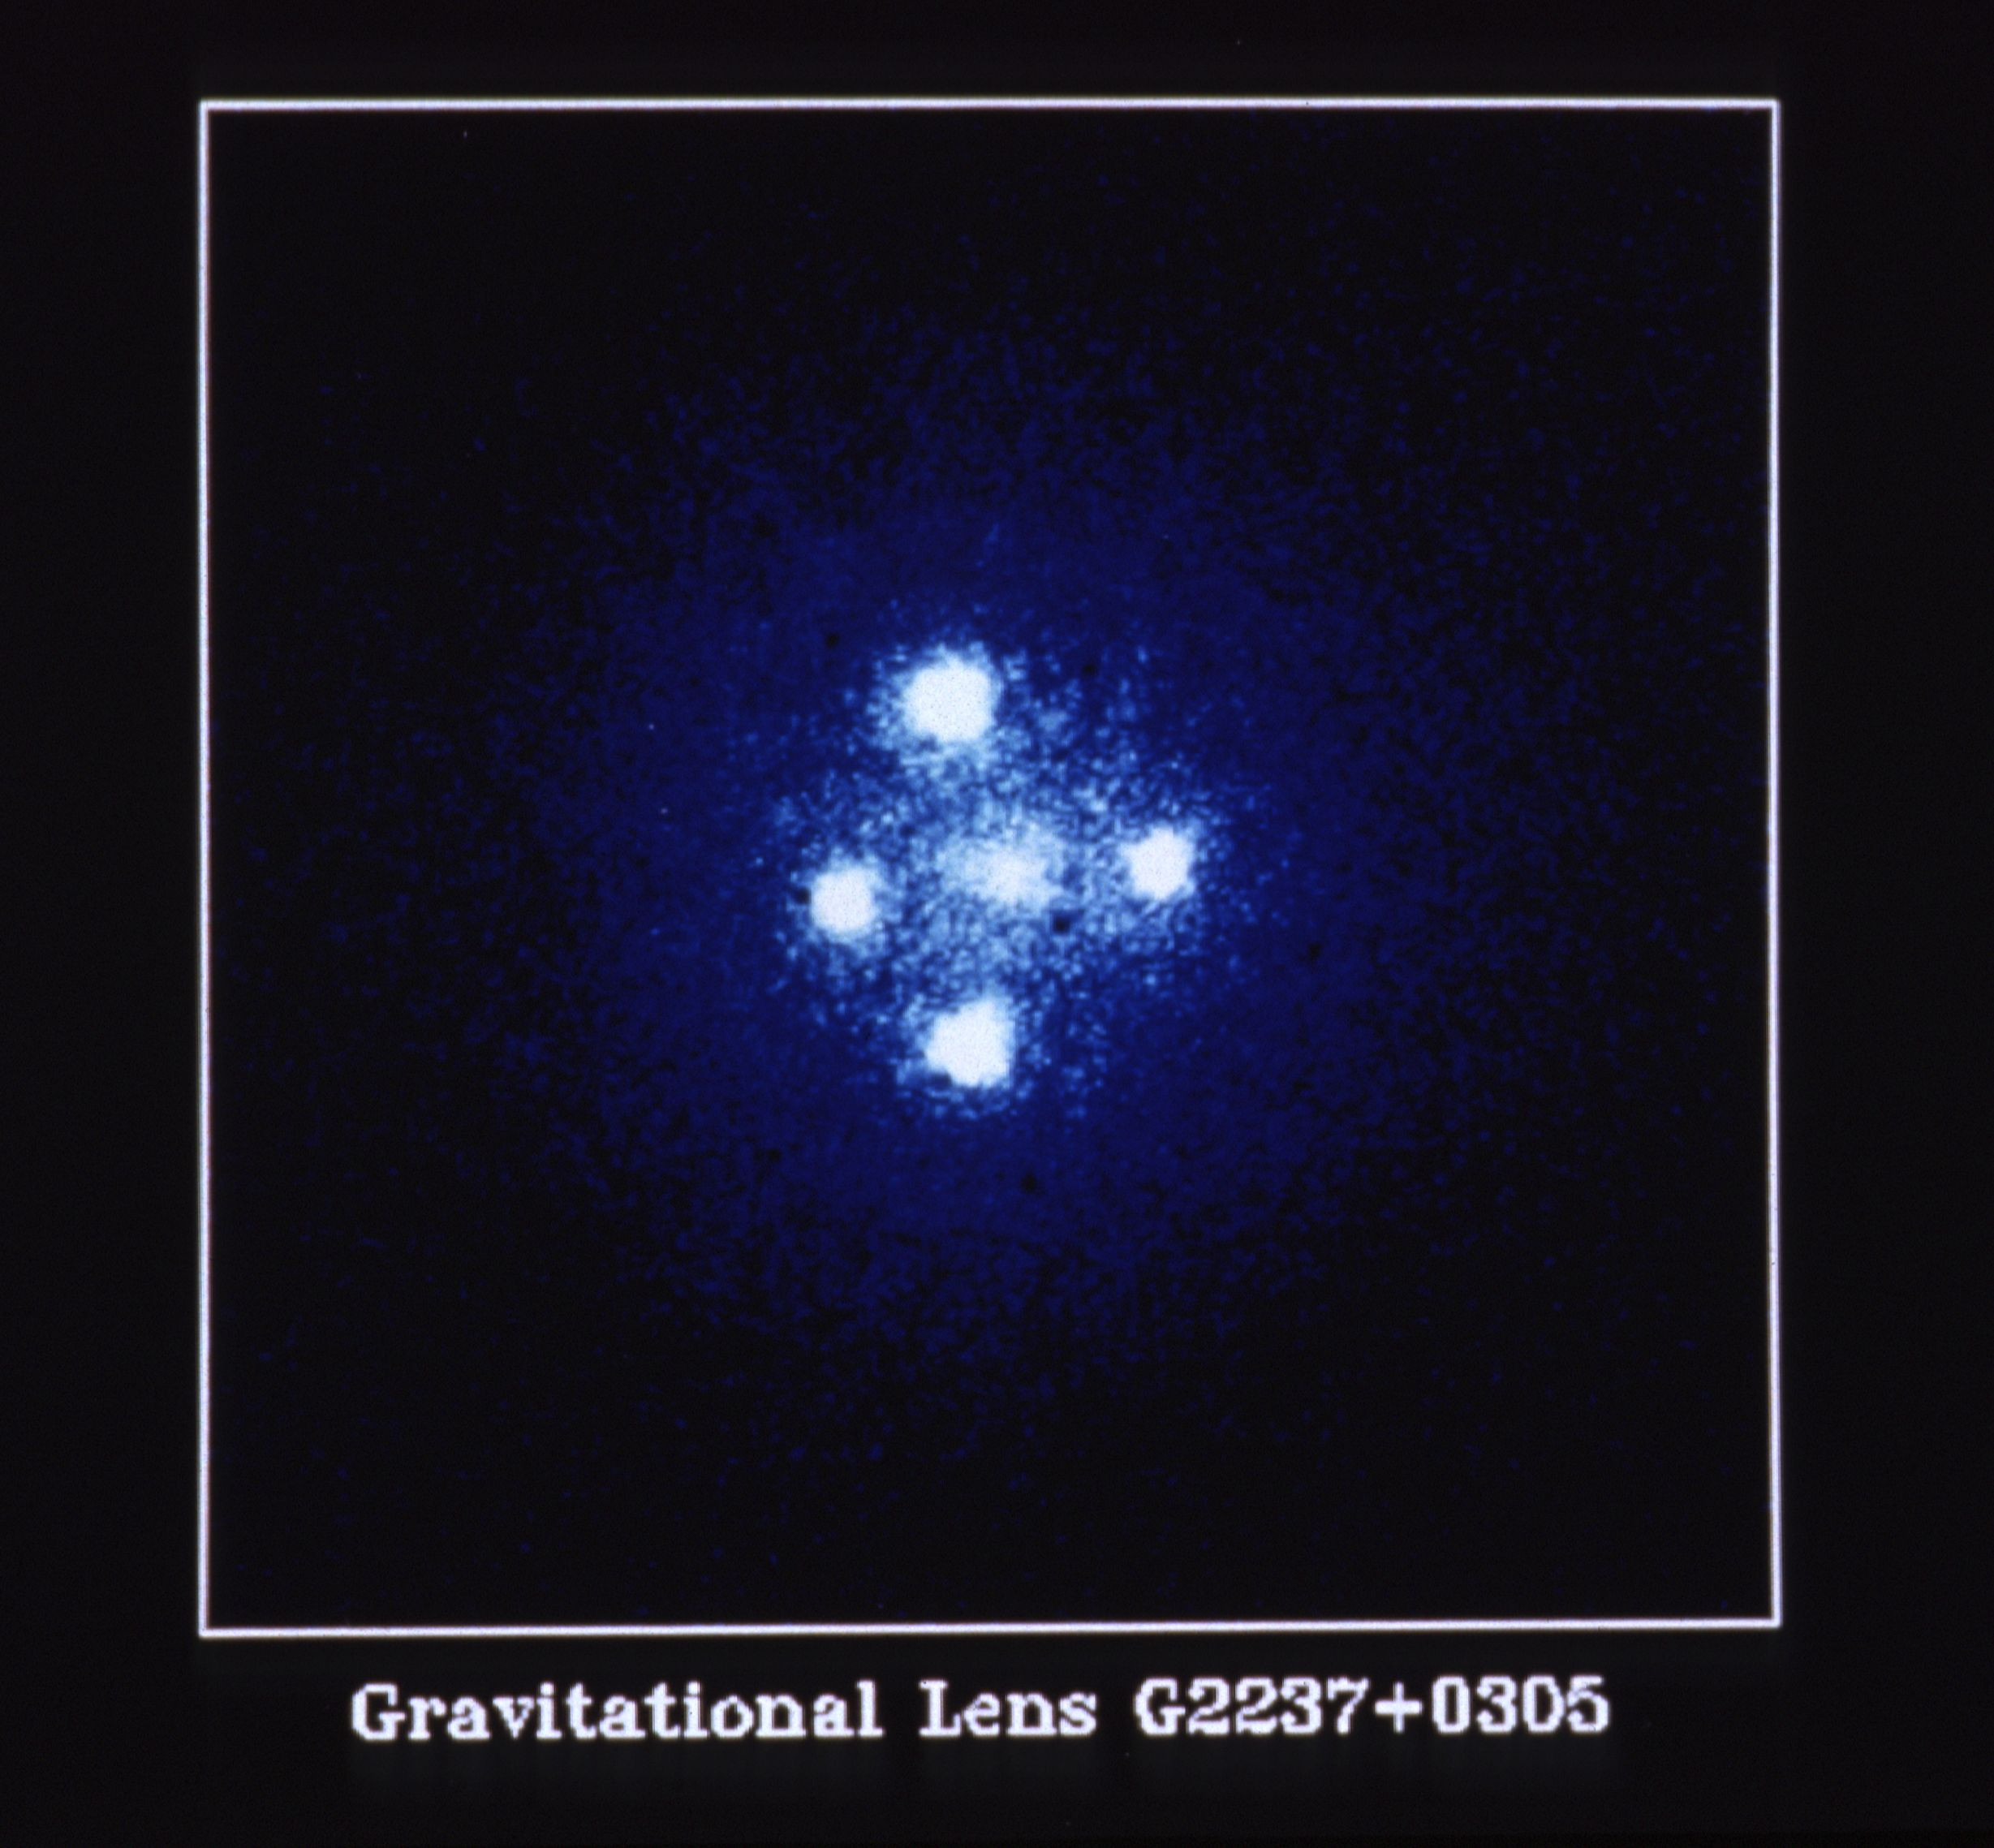
\includegraphics[width=0.8\textwidth]{figures/dm/einstein_cross}
    \caption{The Einstein's Cross, QSO 2237+0305. A distant quasar forms multiple images when lensed around a foreground galaxy. Image from HST~\cite{einstein_cross}.}\label{fig:einstein_cross}
\end{figure}

\subsubsection{Weak lensing}

In cases where the lensing object is not sufficiently dense or massive to create obvious strong lensing, weak lensing can still be observed. Weak lensing can be measured using statistical methods by creating an average shape of a galaxy in the field of view and calculating some distortion parameter~\cite{Bartelmann:1999yn}. A distribution of distortion can be created, which will indicate where the greatest concentrations of mass are. The analysis shows that the amount of mass visible is insufficient to account for the amount of lensing observed.

\subsection{Galaxy cluster dynamics}

\subsubsection{Virial theorem}

Observating the dynamics of clusters of galaxies also yields fairly clear indication that dark matter must form a significant contribution to the mass of a galaxy cluster. When observations are made of clusters other than our own Local Group, a very large mass of diffuse hydrogen is observed in the space between galaxies. This hot gas radiates x-rays (and thus is often called hot x-ray gas), and from its luminosity both the temperature and mass can be measured. The extremely high temperatures observed result from basic energy conservation. As the gas falls into the cluster's gravitational potential well, it gains kinetic energy, which is equivalent to temperature. The temperature of the gas, indicated by its radiation spectrum, thus gives an indication of the depth of the potential well. Applying the Virial theorem (2K~+~U~=~0)~\cite{Claussius:1870} to the cluster, the kinetic energies of the component galaxies can be measured and compared to the potential energy due to the visible mass. In both cases, the required potential well is much deeper than could be formed from merely the hot gas and the galaxies themselves, despite the fact that there is an order of magnitude more mass in gas than in galaxies. Indeed, the extra mass required to make the system behave is an order of magnitude greater than the mass observed in galaxies and gas.

\subsubsection{Bullet cluster}

The Bullet Cluster (1E 0657-558) is an excellent example of both galaxy cluster dynamics and weak lensing, and also furnishes additional information on dark matter. Figure~\ref{fig:bullet_cluster} is a composite image from Hubble Space Telescope (HST), Chandra X-ray Observatory, and Magellan. The pink is the hot x-ray gas (seen by Chandra), and forms the majority of the baryonic mass of the cluster. The powerful shock produced during the collision is clearly seen in the subcluster on the right, giving indications of the speed of the collision, and also the mass of that subcluster. The blue regions, centered on the visible galaxies, show the computed weak lensing centers.

\begin{figure}[htb]
\centering
   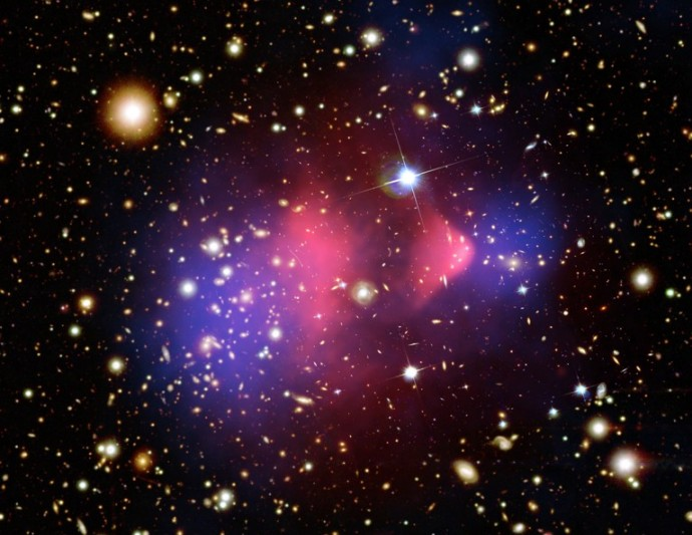
\includegraphics[width=0.8\textwidth]{figures/dm/bullet_cluster}
   \caption{The Bullet Cluster of galaxies, from~\cite{bullet}. Two subclusters passed through each other without significantly affecting the constituent galaxies, however the hot x-ray gas (pink) experienced significant disruption and was pulled away. Despite the majority of visible mass being contained within the gas, a lensing study reveals that the lensing centers (blue) are still centered on the galaxies, indicating that the intracluster gas, while dominating the baryonic mass, is not a major component of the total cluster mass, and also that this invisible matter does not experience significant self-interactions~\cite{Kahlhoefer:2013dca}.}\label{fig:bullet_cluster}
\end{figure}

When the two subclusters passed through each other, the constituent galaxies passed each other with minimal interaction. The two volumes of intracluster gas, being large balls of plasma, experienced significant drag, and the gas separated from the galaxies. A weak lensing study reveals that the lensing centers are still located around the galaxies, even though the mass of the intracluster gas greatly exceeds that of the stars and dust. From this we conclude that the majority of the mass of the subclusters is contained in this invisible matter, and also that it does not experience significant self-interactions~\cite{Kahlhoefer:2013dca}.

\subsection{Structure formation}

After the creation of atoms some $400\,000$ years following the Big Bang, larger structures started forming under the influence of gravity. Any region of slightly higher density started accumulating more matter. This process can be simulated by starting from measurements of the density of the early universe (discussed below) and propagating interactions of gravity and electromagnetism over time. While the computational cost of simulating the universe is, predictably, quite high, this has been done with great success by the Millenium~\cite{Springel:2005nw}, Illustris~\cite{Genel:2014lma,Vogelsberger:2014dza,Sijacki:2014yfa}, and IllustrisTNG~\cite{Pillepich:2017jle} projects. The results found by these simulations is that the large scale structure observed in the universe does not form under the interaction of baryonic matter alone. The inclusion of dark matter is necessary for these structures to form. Indeed, the structures observed in these simulations, as shown in Figure~\ref{fig:structure}, bears very strong resemblance to what is seen with telescopes.

\begin{figure}[htb]
    \centering
    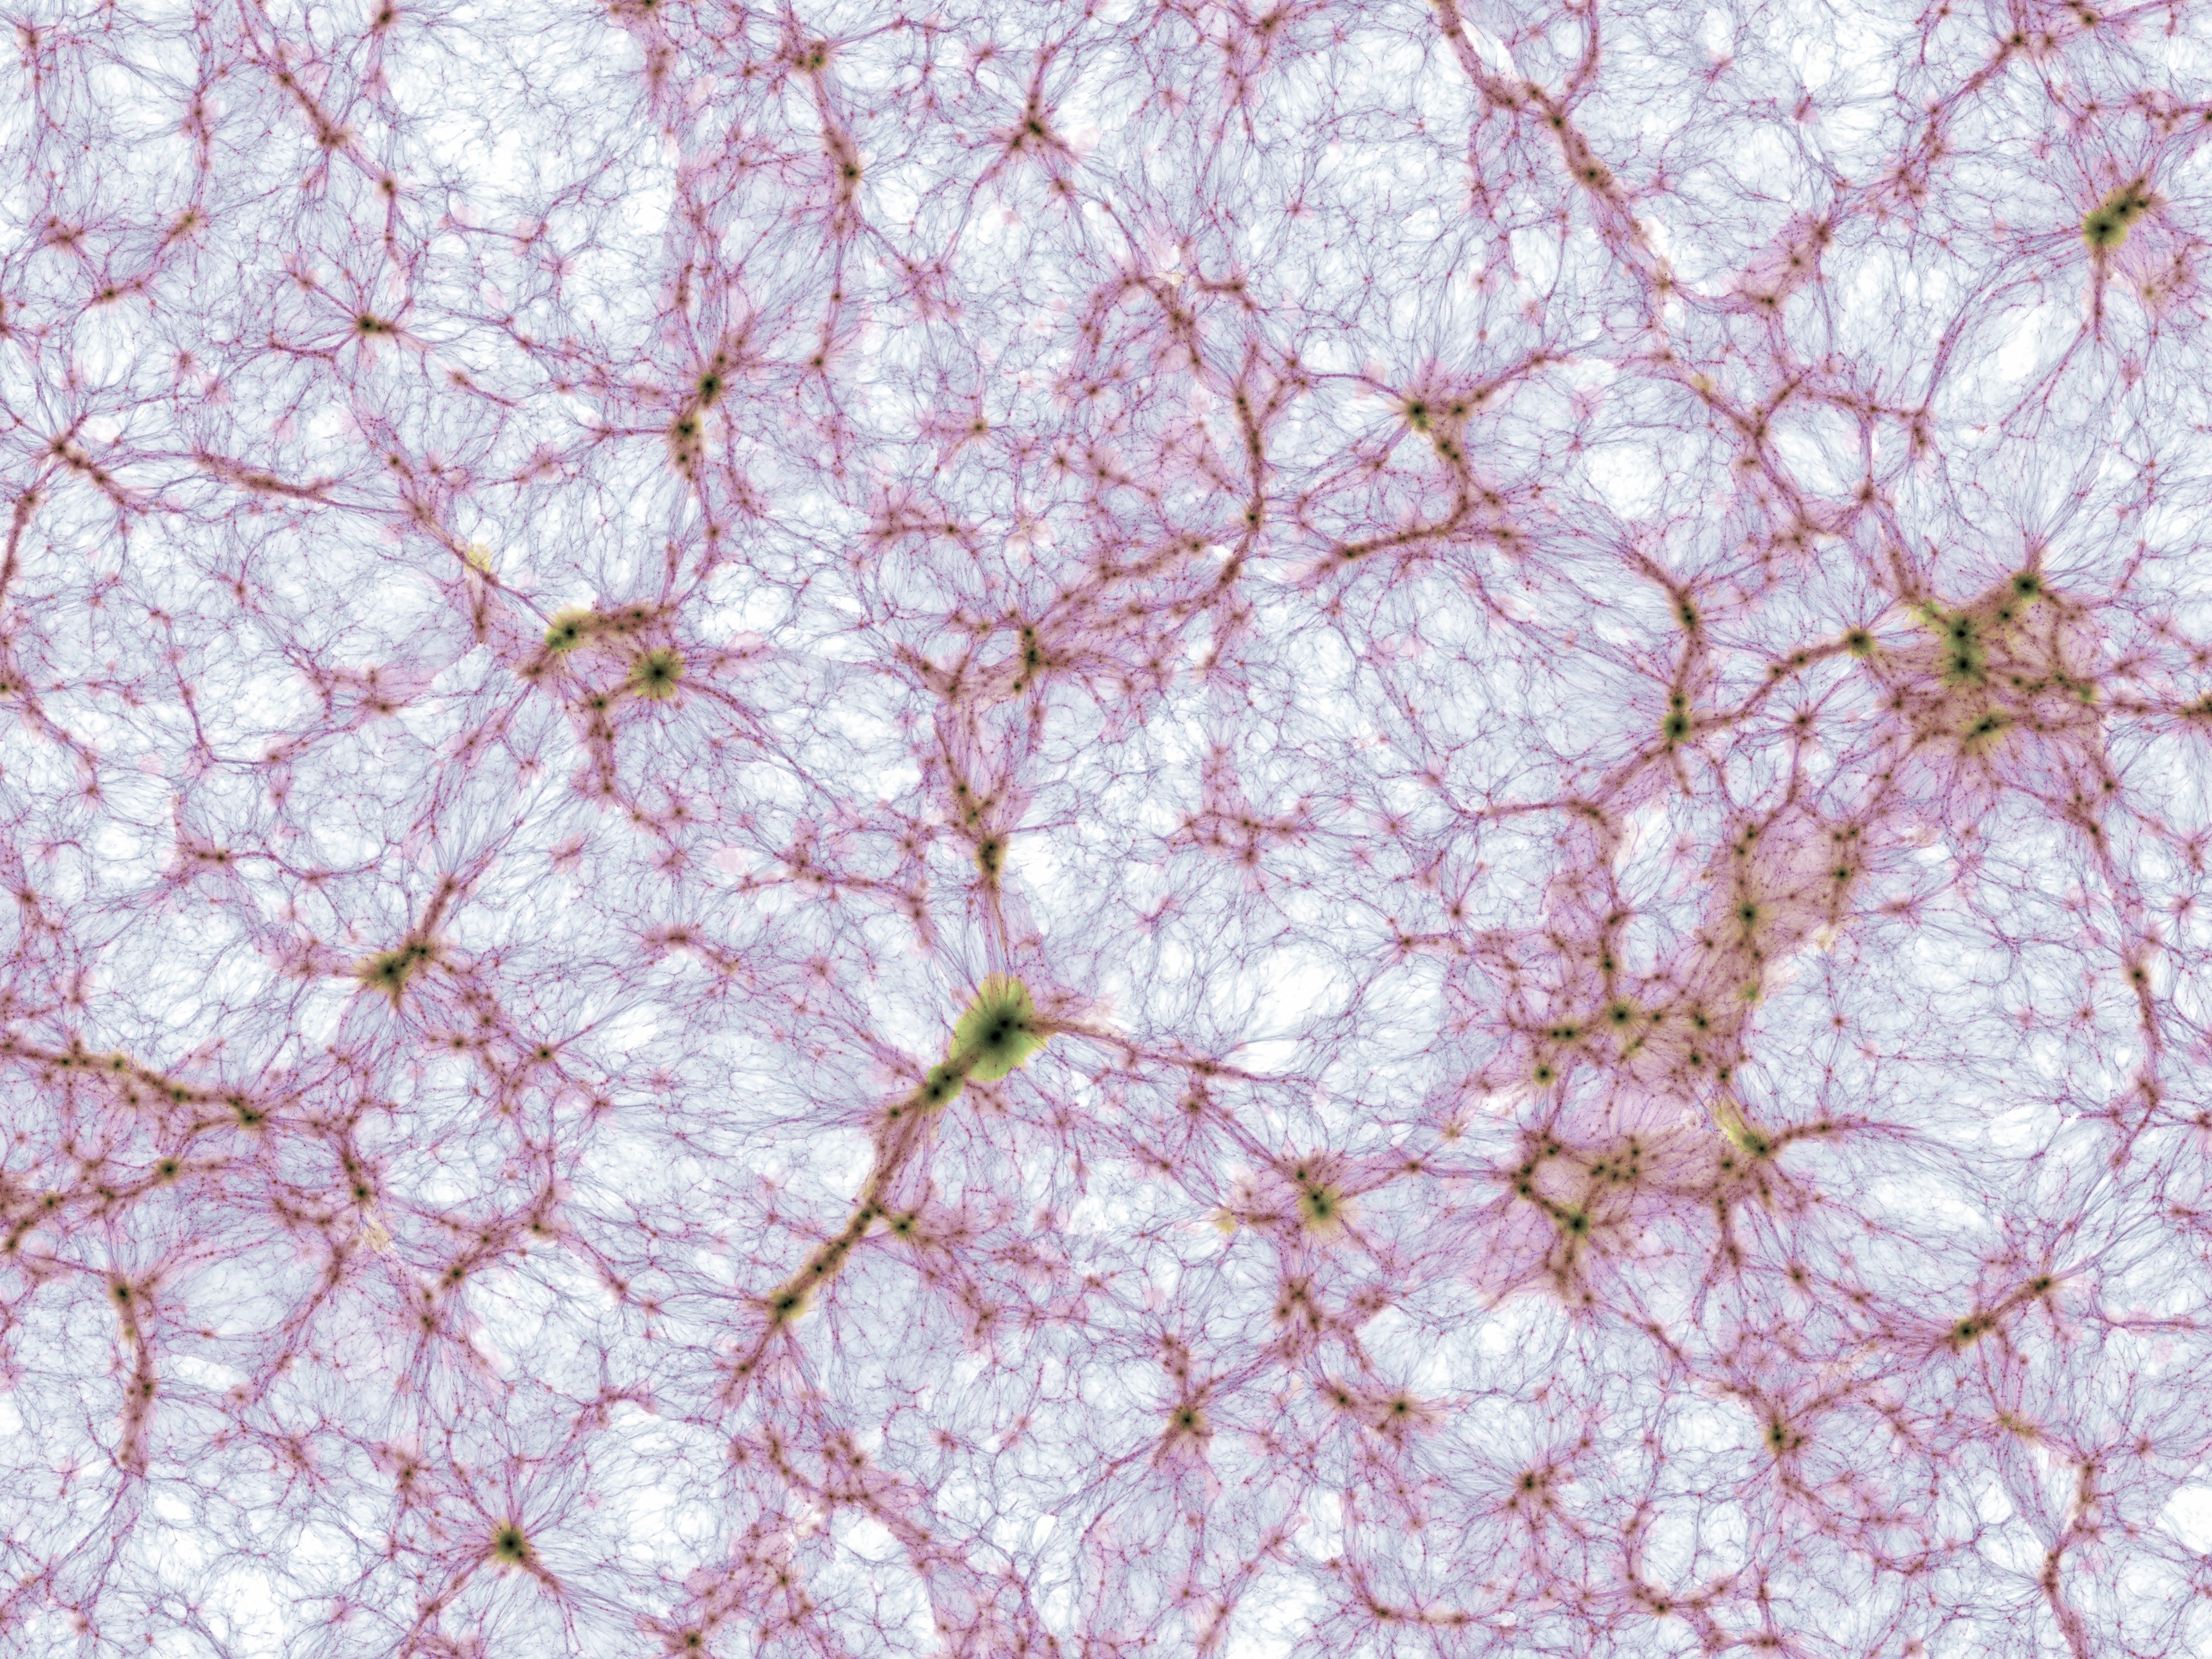
\includegraphics[width=0.8\textwidth]{figures/dm/TNG300_gas_dens_temp_hr}
    \caption{An image from the TNG300 simulation of IllustrisTNG~\cite{Pillepich:2017jle} showing the baryon density and the gas temperature. Without the inclusion of a significant quantity of dark matter, the kind of structure observed in the universe does not form.}\label{fig:structure}
\end{figure}

\subsection{Cosmic Microwave Background (CMB)}

Penzias and Wilson were the first to turn a sensitive microwave telescope to the skies~\cite{Penzias:1965a,Penzias:1965b}, and their discovery earned them the Nobel Prize in Physics in 1978. The best measurements of the CMB come from satellites like Wilkinson Microwave Anisotropy Probe (WMAP)~\cite{Bennett:2012zja} and Planck~\cite{Ade:2015xua}, and are (at face value) nearly totally featureless and isotropic to a few parts per million as shown in Fig.~\ref{fig:cmb}a. After the subtraction of the average, dipole, and galactic contributions, we get Fig.~\ref{fig:cmb}b.

\begin{figure}[htb]
    \begin{tabular}{cc}
    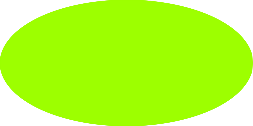
\includegraphics[width=0.5\textwidth]{figures/dm/CMB0} & 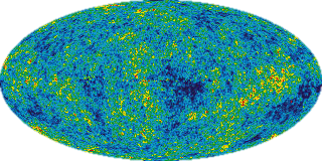
\includegraphics[width=0.5\textwidth]{figures/dm/CMB3} \\
    \end{tabular}
    \caption{(Left) The cosmic microwave background radiation as measured by WMAP~\cite{Bennett:2012zja}. The temperature of the universe is flat and lacking any features above the a few parts per million. (Right) After subtracting the contributions from various backgrounds, we see the temperature profile of the universe at the moment when photons decoupled from baryons about $380\,000$ years after the Big Bang. Hotter regions had a greater concentration of the primordial soup and formed from quantum fluctuations in the early universe.}\label{fig:cmb}
\end{figure}

Certain regions radiate at a slightly higher temperature, indicating a greater concentration of the soup of baryons and photons in the early universe. These differences arose due to quantum fluctuations during the early expansion. This temperature map can be expanded in the spherical harmonics and a power spectrum plotted. Various cosmological models can be tested by fitting to this spectrum, as shown in Figure~\ref{fig:cmb_ps}.

\begin{figure}[htb]
\centering
    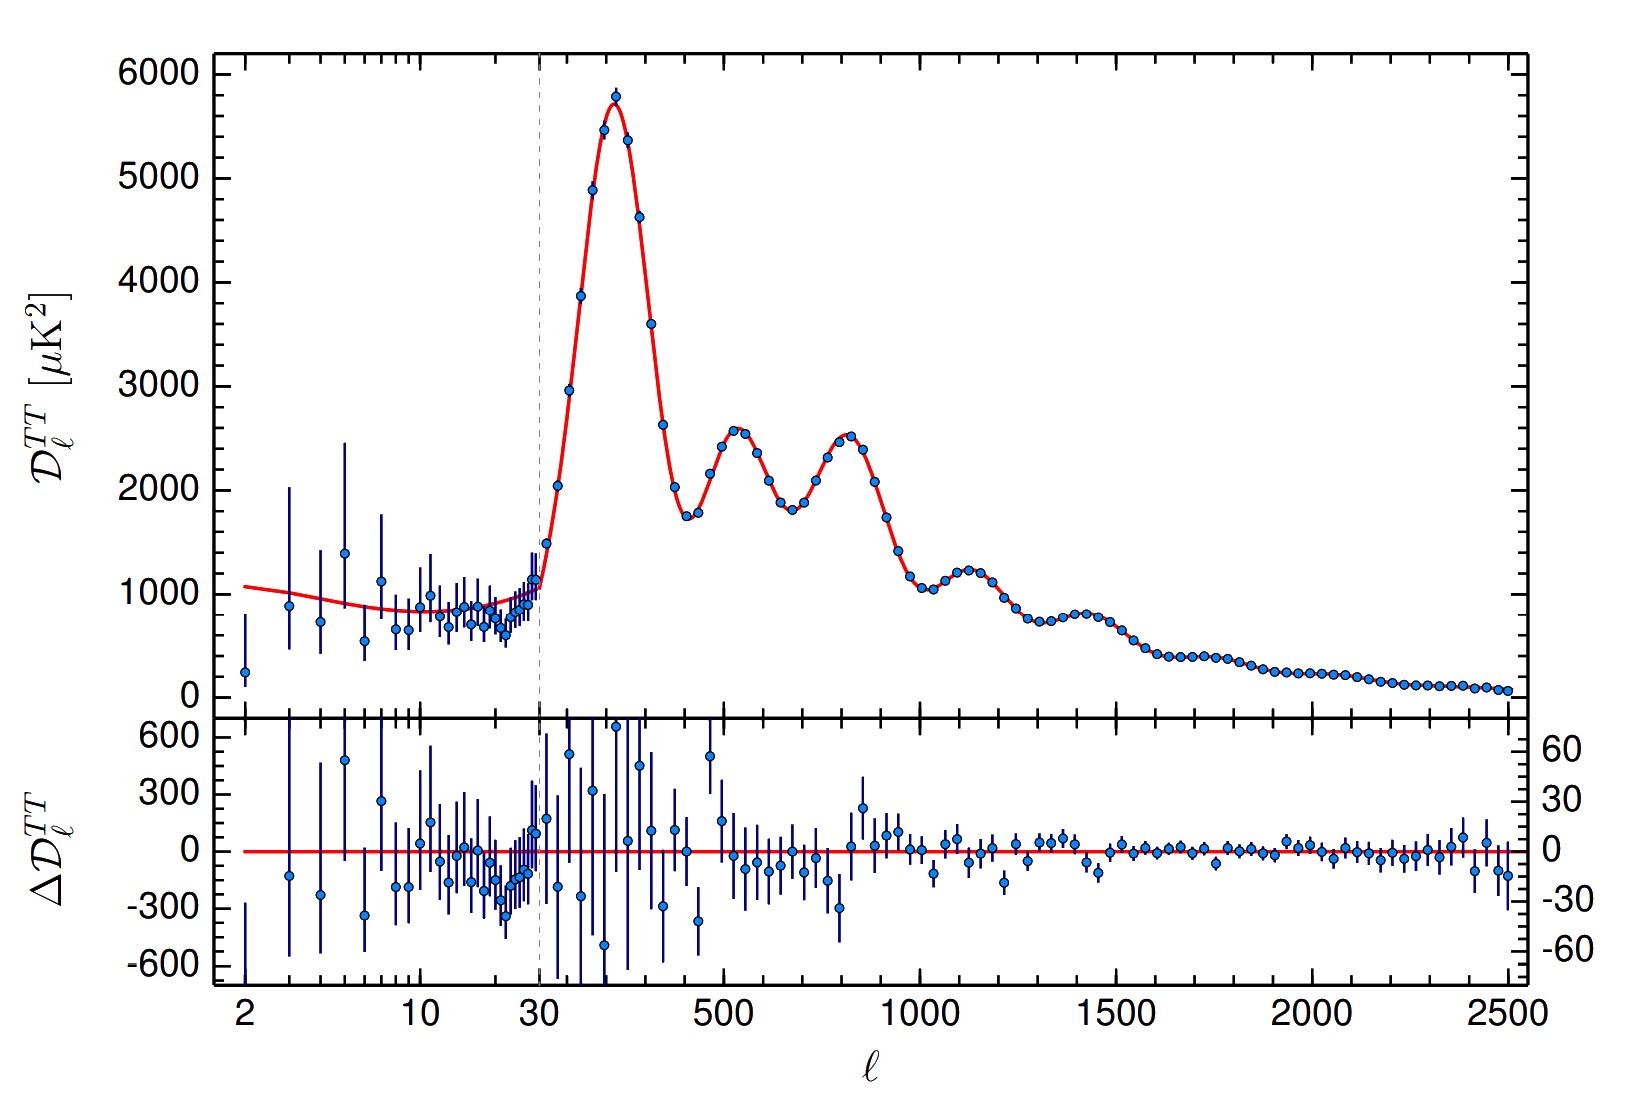
\includegraphics[width=0.8\textwidth]{figures/dm/planck2015_cmb}
    \caption{The power spectrum of the spherical harmonic expansion of the CMB from Planck~\cite{Ade:2015xua}. The lack of damping on the second peak indicates significant contributions to the universe from non-baryonic matter.}\label{fig:cmb_ps}
\end{figure}

The model with the best fit is $\Lambda$CDM, which at its simplest is a six-parameter model that describes the universe as filled with cold (non-relativistic) dark matter (CDM) with additional contributions from dark energy ($\Lambda$)~\cite{Riess:1998cb}. From the results extracted from the fit we learn a variety of things about the universe. Of key importance are the various contributions to the total energy content of the universe. According to Planck~\cite{Ade:2015xua}, the baryonic fraction $\Omega_b$ is merely $0.049$, the dark matter fraction $\Omega_{\n{DM}}$ $0.265$, and the dark energy fraction $\Omega_{\Lambda}$ $0.686$. Thus, the majority of the universe is not of a baryonic nature.

\subsection{Big Bang Nucleosynthesis (BBN)}

Within a minute after the Big Bang, the universe had cooled sufficiently to allow nuclei to form and not be immediately broken apart due to the high ambient temperature. Neutrons and protons had just fallen out of numerical equilibrium due to their small difference in mass, and now existed in a ratio of about 1 neutron per 7 protons. Neutrons and protons first combined to make deuterium, then as the deuterium abundance increased, deuterium fused with deuterium to produce tritium and helium-3 and then with tritium to produce helium-4. This epoch continued for just under half an hour, until expansion had driven particles far enough apart that collisions became infrequent and cooling robbed the collisions of sufficient energy to initiate the reactions. At this point, the majority of the universe's neutrons were in helium due to its stability, and of the few remaining, most were in deuterium. Due to the weak binding of deuterium, a universe with more photons will mean fewer deuterium nuclei survive this epoch. Due to its stability, the population of $^4$He depends very little on the photon density. By measuring the primordial abundance of deuterium, this will admit a value of the ratio between nuclei and photons, which will in turn indicate what percentage of the universe was baryonic in this epoch.

By comparing the prediction from theory with measurements (Ref~\cite{Steigman:2007xt}, see also Figure~\ref{fig:bbn}), we can place a stringent requirement on the baryonic density of the universe to $\eta = (6.11\pm2.0)\times10^{-10}$, where $\eta$ is the ratio between the number of baryons and photons. This value of $\eta$ indicates that the majority of the universe is not of a baryonic nature.

\begin{figure}[htbp]
\centering
    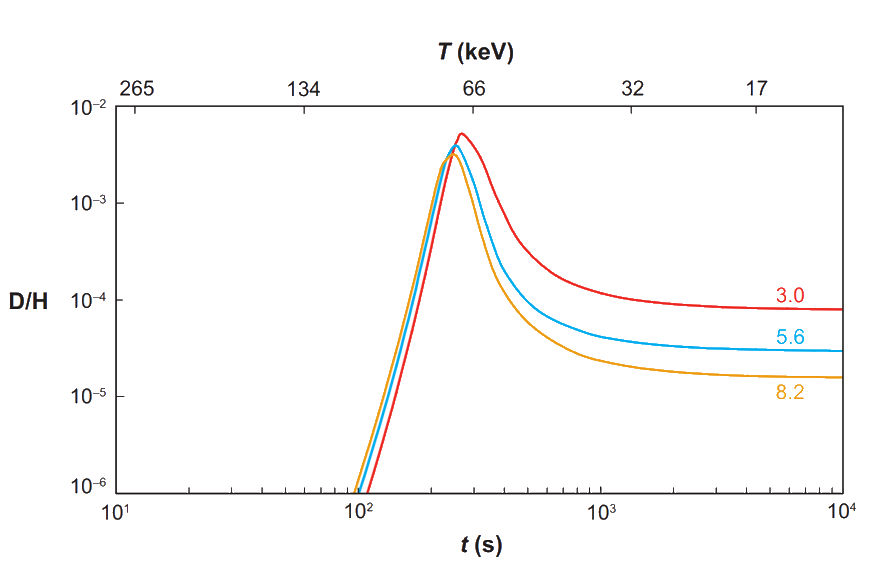
\includegraphics[width=\textwidth]{figures/dm/bbn_eta}
    \caption{The evolution of the relative abundance of deuterium depends strongly on the ratio between baryons and photons in the early universe. Deuterium forms from hydrogen, then combines with deuterium to form helium-3 and tritium or with tritium to form helium-4. Due its weak binding, deuterium is an excellent probe of the photon density. Measuring the deuterium abundance in the early universe admits a value of the baryon density during this epoch, which indicates that only a small fraction of the universe is baryonic. Figure from~\cite{Steigman:2007xt}.}\label{fig:bbn}
\end{figure}

\section{Searching for Dark Matter}

To search for dark matter, we need some ideas of what to look for. While we don't know what dark matter is, we can still start from things we already know about astrophysics and particle physics. We know any dark matter must be gravitationally bound to the Milky Way, which limits the maximum velocity to be escape velocity from the galaxy $v_{esc} \approx 600\1{km/s}$. Moreover, we know that dark matter does not experience significant self-interactions, and must have a long lifetime compared to the age of the universe. Additionally, we know that there must be some physics beyond the Standard Model.

The traditional approach has been to assume strong priors from both cosmology and particle physics, where a thermal relic particle and weak-scale physics beyond the standard model (BSM) like supersymmetry combine to give to the Weakly Interacting Massive Particle (WIMP)~\cite{Jungman:1995df}, on which we will primarily focus.

If we relax the strong particle physics prior, we have a generic thermal or quasi-thermal relic particle.

Relaxing just the cosmological physics prior proposes the QCD axion, first proposed to solve the strong CP problem~\cite{Peccei:1977,Weinberg:1978,Wilczek:1978}, as a dark matter candidate. Despite having very low masses ($10^{-12}\1{eV}$ to $10^{-2}\1{eV}$), the production mechanism of axions~\cite{Preskill:1983,Abbott:1983,Dine:1983} allows them to be created cold.

By assuming some unknown interaction mechanism between dark matter particles and standard model particles, we can draw a Feynman diagram to represent possible ways to investigate the nature of dark matter, as shown in Figure~\ref{fig:feynman}.

\begin{figure}[htb]
    \centering
    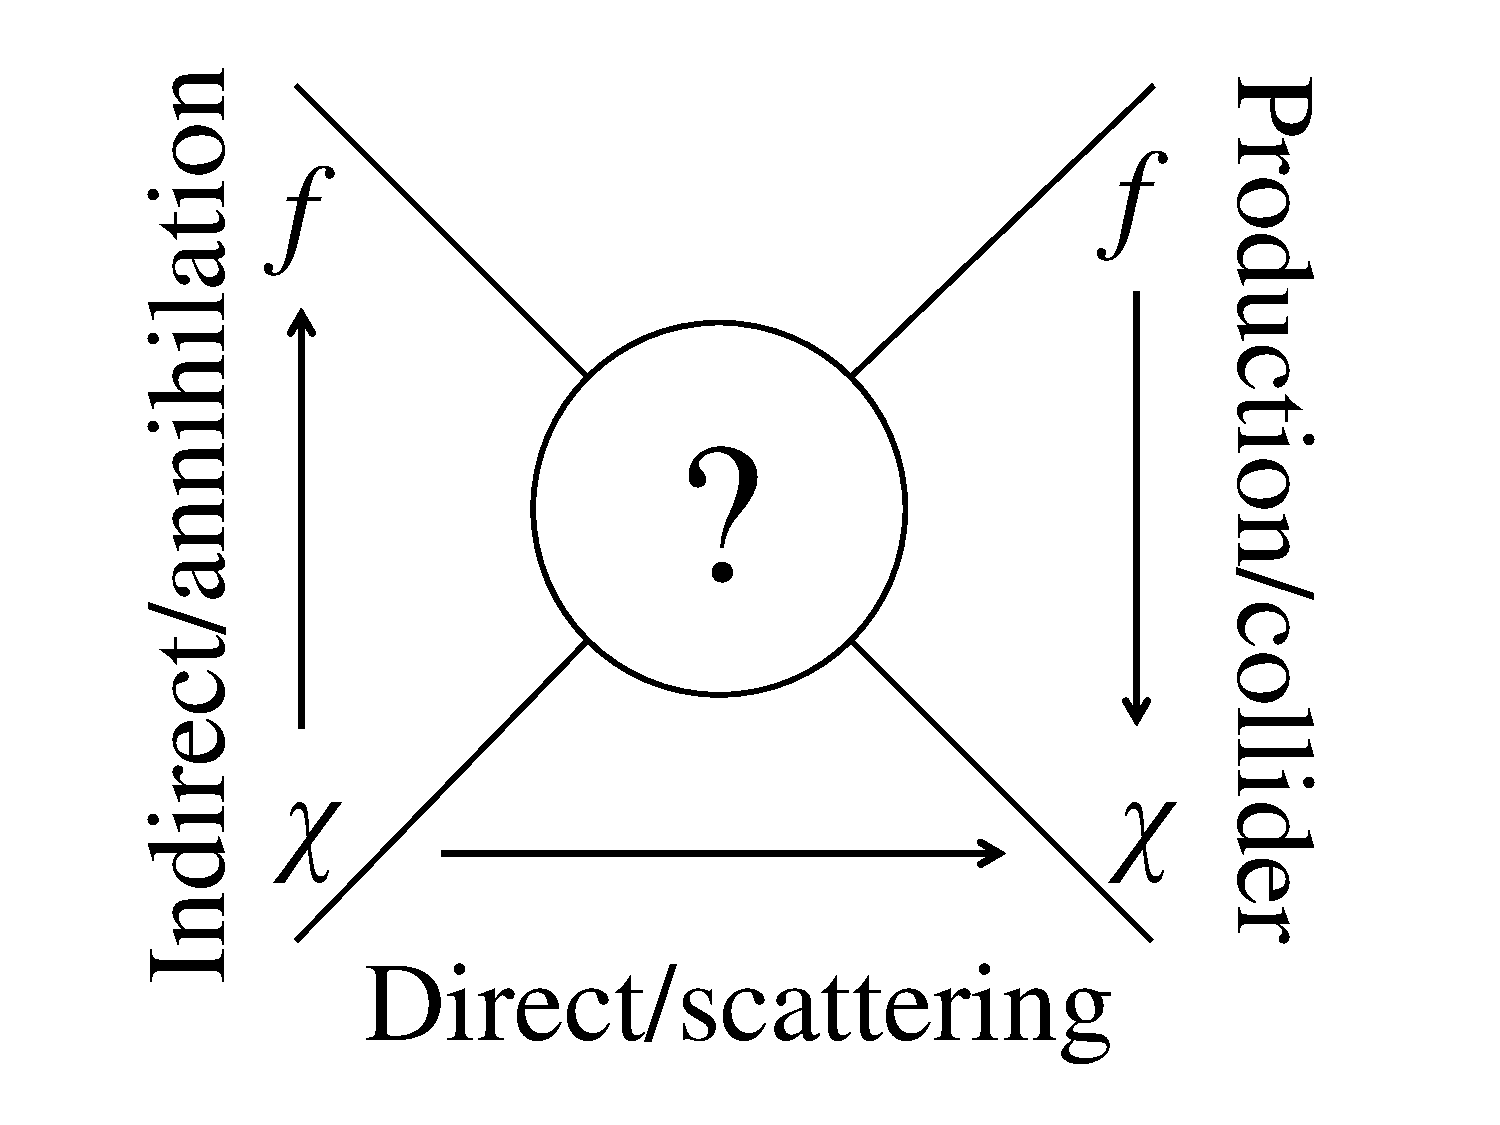
\includegraphics[width=0.8\textwidth]{figures/dm/feynman_diag}
    \caption{A Feynman diagram showing possible interactions between a Standard Model fermion \textit{f} and a dark matter particle $\chi$, and three different search methodologies.}\label{fig:feynman}
\end{figure}

\subsection{Production Searches}

Attempts to produce dark matter at colliders are led by the CMS~\cite{cms:2008} and ATLAS~\cite{atlas:2008} experiments at the LHC, following the interaction along the right side of Figure~\ref{fig:feynman}. Various parameter spaces are searched for the signatures of new particles, for instance the Higgs boson~\cite{cms:2012,atlas:2012}. Because any dark matter particle produced in the collision between (for instance) two protons is not expected to interact with a detector before escaping, the experimental signature of such an event would be missing momentum. Several searches for this signature have been performed, but the results so far are consistent with Standard Model expectations~\cite{atlas:2016,cms:2017}.

\subsection{Annihilation Searches}

In a region with higher dark matter density, such as galactic centers, the probability increases for any two dark matter particles to have some interaction with each other. Following the left side of Figure~\ref{fig:feynman}, two dark matter particles that annihilate could create a pair of standard model particles, which a detector could observe. Many experiments are engaged in these searches, including AMS~\cite{Aguilar:2013} and Fermi-LAT~\cite{Ackermann:2013uma} in space, and HESS~\cite{Abramowski:2014tra}, VERITAS~\cite{Arlen:2012}, and MAGIC~\cite{Aleksic:2013xea} on land, to name but a few. While occasional signals are seen at some significance, such as the $3.5\1{keV}$ line~\cite{Boyarsky:2014jta,Bulbul:2014sua} observed in 2014, astrophysical sources have been proposed and a concensus on the origin of these signals has not been reached~\cite{Shah:2016efh,Ahnen:2016qkx,Abdallah:2016ygi,Archambault:2017wyh,Albert:2016uux}.

\subsection{Scattering Searches}

The final interaction to discuss is the bottom of Figure~\ref{fig:feynman}. Here, a dark matter particle scatters off a target particle, imparting some momentum to the target. The three types of signals from these interactions are phonons, photons, and electron/hole pairs. Most detectors are designed to collect two of these three, leading to a wide variety of detector materials, designs, and configuration. These include crystals and bolometers, both semiconducting and inorganic, (CDMS~\cite{Akerib:2005,Agnese:2015ywx}, CRESST~\cite{Kluck:2017hnn}, and EDELWEISS~\cite{Armengaud:2009hc,Armengaud:2017rzu}), bubble chambers with superheated liquids (PICO~\cite{Amole:2015pla,Amole:2017dex} and COUPP~\cite{Manuel:2016klm}), noble liquid scintillation counters (DEAP~\cite{Amaudruz:2017ibl,Amaudruz:2017ekt} with argon, XMASS~\cite{Abe:2013tc} with xenon), and dual-phase noble time projection chambers (TPCs) (DarkSide~\cite{Agnes:2014bvk,Agnes:2015ftt} and ArDM~\cite{Marchionni:2010fi,Calvo:2015uln,Calvo:2016hve} using argon, and XENON10~\cite{Angle:2007uj}, ZEPLIN~\cite{Akimov:2011tj}, XENON100~\cite{Aprile:2011dd,Aprile:2013doa}, LUX~\cite{Akerib:2013tjd}, PandaX-II~\cite{Cui:2017nnn}, and XENON1T~\cite{Aprile:2017aty} using xenon). The easier scalability of noble liquid detectors over crystals makes them the dominant technology, and they continue to push to greater sensitivities. In these direct detection experiments, the usual parameter space to report results is that of the WIMP-nucleon scattering cross section versus the WIMP mass, as shown in Figure~\ref{fig:limits}. As no verified signals have been observed, experiments continue to place upper limits on in this space. We will focus on XENON1T, but much of this discussion applies to all direct detection experiments.

\begin{figure}[htb]
    \centering
    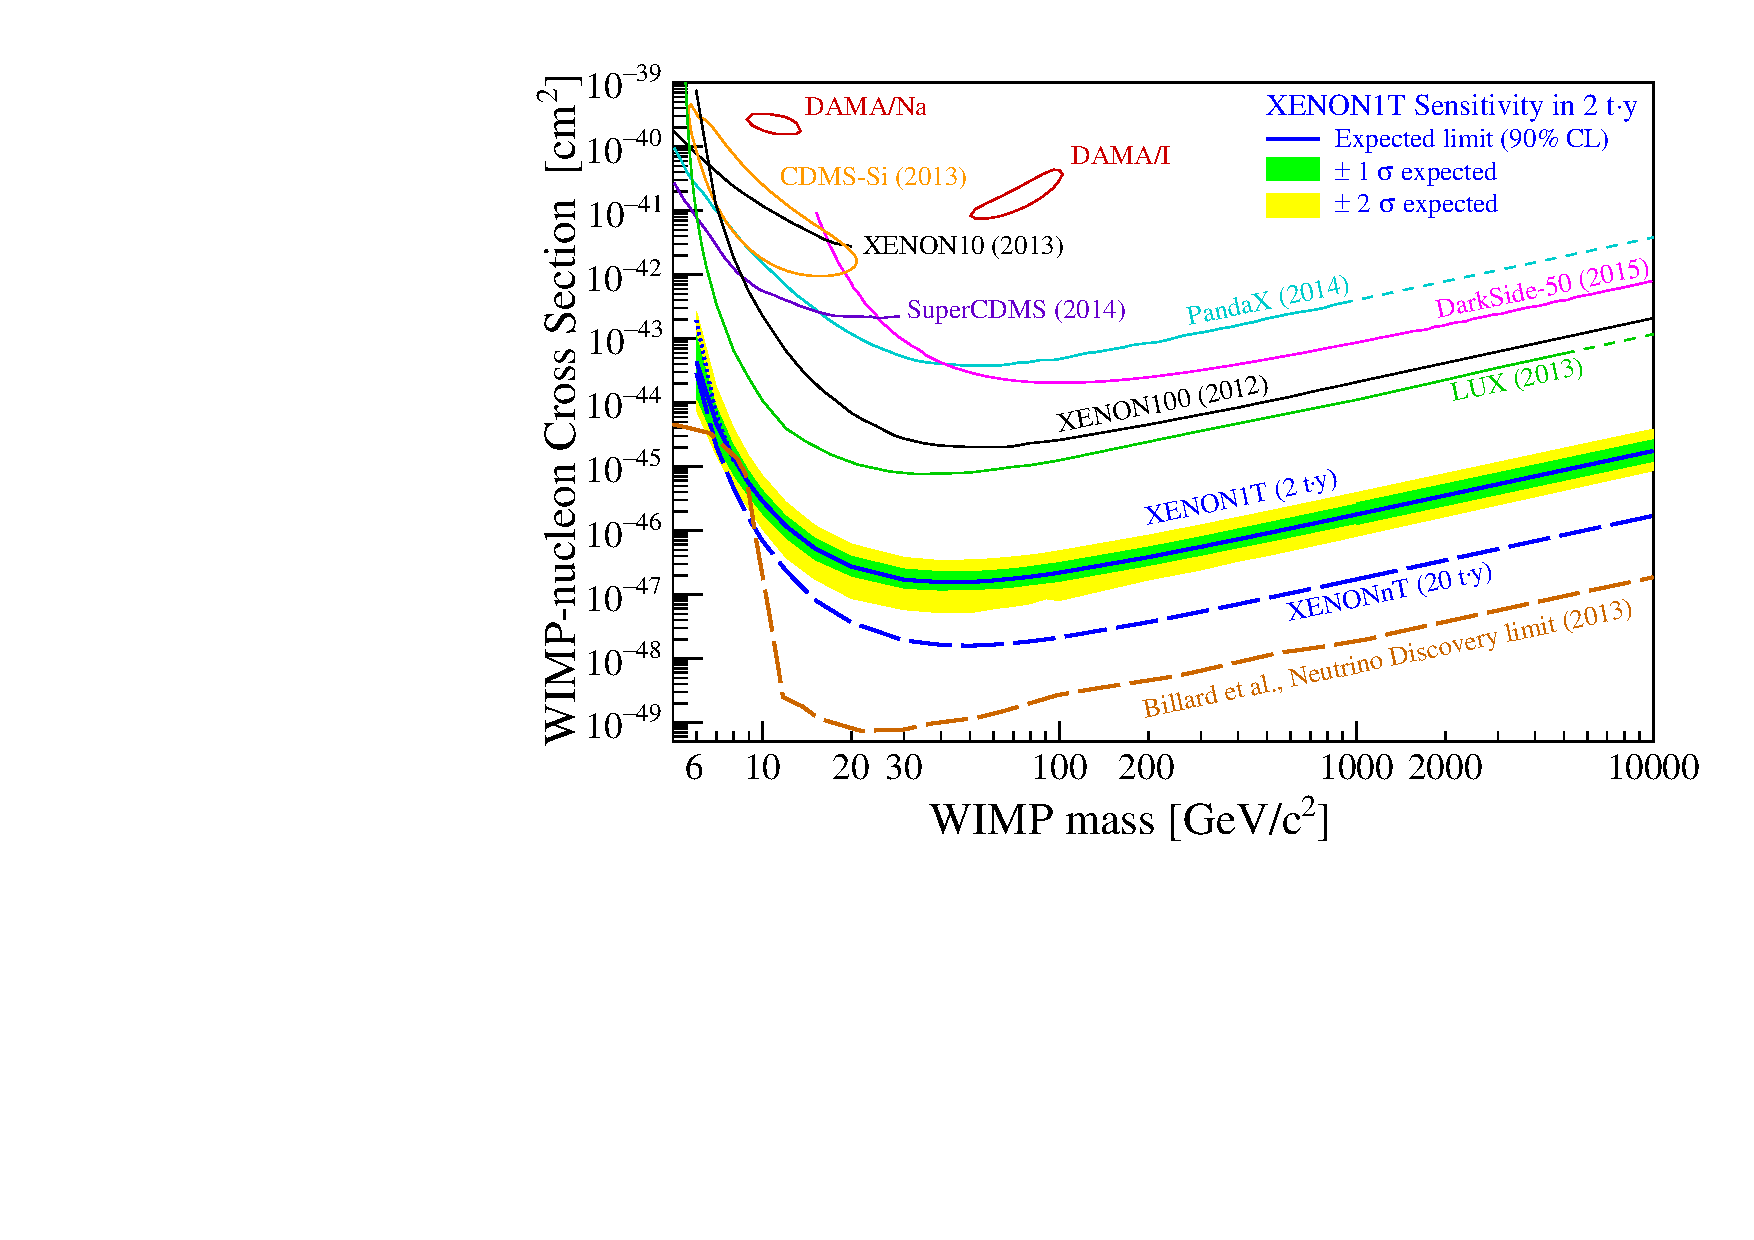
\includegraphics[width=0.8\textwidth]{figures/dm/limit_plot}
    \caption{Expected sensitivity of XENON1T to the spin-independent WIMP-nucleon scattering cross section, from~\cite{Aprile:2015uzo}. Included are results and exclusion limits from DAMA-LIBRA~\cite{Savage:2008er}, CDMS-SI~\cite{Agnese:2013rvf}, XENON10~\cite{Angle:2013}, SuperCDMS~\cite{Agnese:2014aze}, PandaX~\cite{Xiao:2014}, DarkSide-50~\cite{Agnes:2015ftt}, XENON100~\cite{Aprile:2012nq}, and LUX~\cite{Akerib:2015rjg}. The background due to coherent neutrino-nuclear scattering is from~\cite{Billard:2013qya}. The scalability of liquid noble detectors, especially those using xenon, have significantly outpaced semiconductors above a dark matter mass of a few GeV. Also shown is the projected sensitivity for the XENONnT detector upgrade. The decrease of sensitivity to lower mass dark matter arises from the reduced energy deposition in an interaction and the difficulty of detecting these smaller signals; the decrease towards higher mass is due to the decreasing dark matter number density and flux.}\label{fig:limits}
\end{figure}

There are a number of other topics important to direct detection experiments to discuss, such as backgrounds and the specifics of the expected signals.

\subsubsection{Backgrounds}

The limiting factor of any experiment is the background to the signal of interest. As the expected signature of a WIMP interaction is a low-energy nuclear recoil (NR), any process that also produces this is a potential background. Sources of neutrons, then, are especially dangerous. The three dominant sources of neutrons and nuclear recoil events for XENON1T are radiogenic and cosmogenic neutrons, and coherent elastic neutrino-nuclear scattering (CEvNS)~\cite{Freedman:1977,Scholberg:2015,Billard:2013qya}. Radiogenic neutrons are due to the $(\alpha,n)$ reaction and spontaneous fission of uranium and thorium contaminants in detector materials; cosmogenic neutrons are caused by muon-induced spallation, and CEvNS events are primarily due to neutrinos produced by $^8$B in the solar core. Taken together, the expected nuclear recoil background rate in the range (4,~50) $\n{keV}_{nr}$ in XENON1T is $(0.6 \pm 0.1)\1{(t\cdot y)^{-1}}$~\cite{Aprile:2015uzo}, predominantly from the radiogenic neutrons. Below 3~$\n{keV}_{nr}$ the rate from CEvNS increases significantly, rising to $\sim 90\1{(t\cdot y)^{-1}}$ at a 1~keV threshold.

Additionally, there are backgrounds rising from electronic recoils (ER) that leak into the nuclear recoil region of interest. Because the discrimination between electronic and nuclear recoils for most detectors is merely good and not perfect, an ER rejection level of $99.5\%$ means $0.5\%$ of ER events will leak into the NR band. The major sources of ER events are low-energy $\beta$ decays of \Pb~(one of the daughters of \Rn) and $^{85}$Kr, solar neutrinos from the $pp$ process that scatter off electrons, Compton scatters from $\gamma$s emitted by contaminants in the materials, and low-energy $2\nu\beta\beta$ decays of $^{136}$Xe, as shown in Figure~\ref{fig:er_bkg}.

\begin{figure}[htb]
\centering
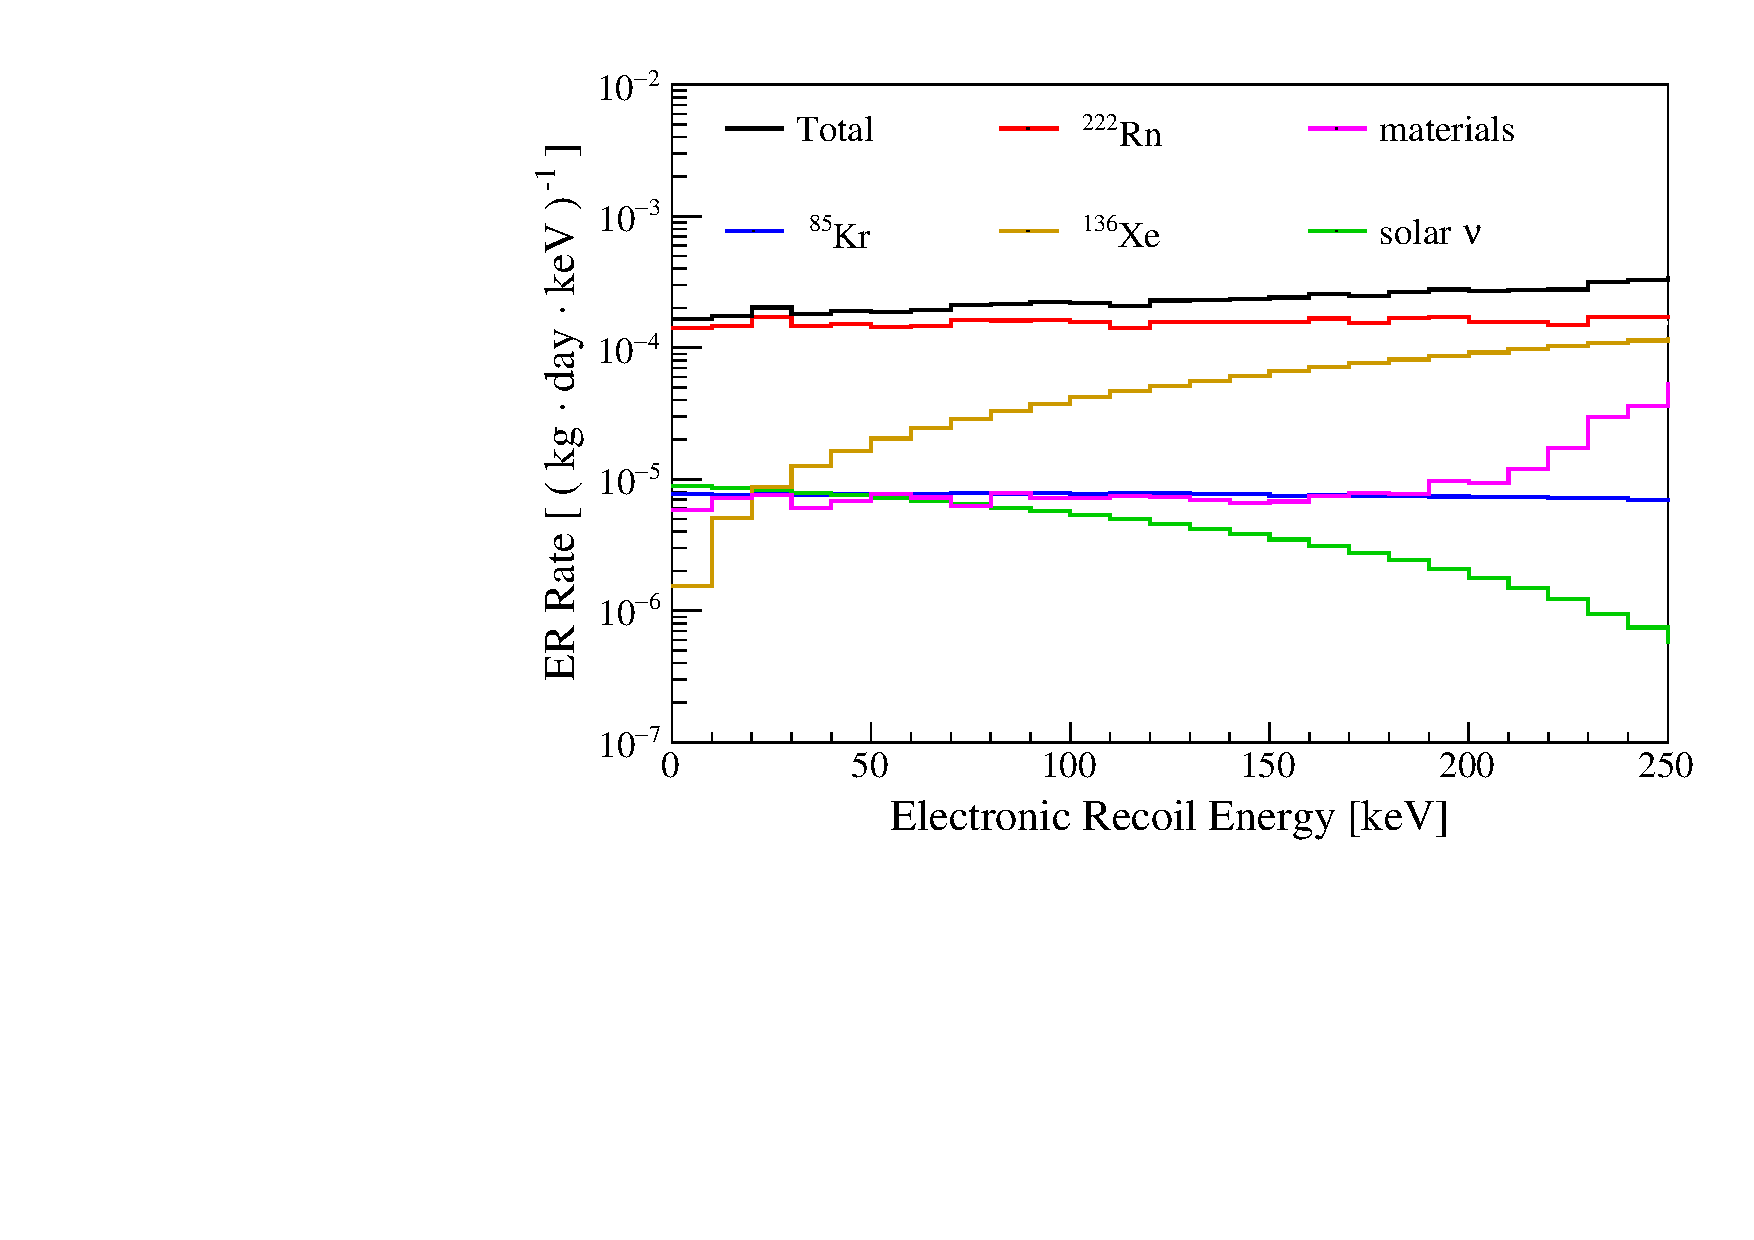
\includegraphics[width=0.8\textwidth]{figures/dm/er_bkg_low}
\caption{The simulated low-energy electronic recoil background spectrum in the XENON1T fiducial volume. The energy region of interest for dark matter events is the first bin. The concentration of \Rn~is $10\1{\mu Bq/kg}$ and of Kr is $<0.2\1{ppt}$. The $^{136}$Xe abundance is assumed to be natural. Figure from~\cite{Aprile:2015uzo}.}\label{fig:er_bkg}
\end{figure}

The background from krypton can be mitigated by removing krypton through cryogenic distillation~\cite{Aprile:2016xhi} and the backgrounds from \Rn~and material components by careful material screening and selection~\cite{Aprile:2017ilq}. $^{136}$Xe can be removed by the depletion/enrichment processes used commonly for nuclear power. Neutrino backgrounds are, obviously, impossible to shield against or reduce, and represent fundamental limitations to the search for dark matter. The assumed values for XENON1T are a \Rn~concentration of $10\1{\mu Bq/kg}$ and Kr of $<0.2\1{ppt}$ (of which the $^{85}$Kr abundance is $2\times10^{-11}$). This gives XENON1T the lowest background rate of any dark matter experiment of $0.1\1{counts~(keV\cdot tonne\cdot day)^{-1}}$.

\subsubsection{Energy spectrum}

To calculate the expected spectrum of energy deposited in a detector, we combine information about the density $\rho_0$ and velocity distribution $f(v,t)$ of galactic dark matter, the differential scattering cross-section $\dd\sigma/\dd E(E,v)$, and the mass of the target and dark matter particles $m_A$ and $m_{\chi}$, respectively, as described in (for example)~\cite{Undagoitia:2015gya,Lewin:1996}:
\begin{equation}\label{eq:recoil_spectrum}
\frac{\dd R}{\dd E}(E,t) = \frac{\rho_0}{m_A \cdot m_{\chi}} \int\dd^3v\,v\,f(v,t)\frac{\dd\sigma}{\dd E}(E,v)
\end{equation}

The time dependence of equation~\eqref{eq:recoil_spectrum} arises due to the motion of the earth around the sun (and, to a much lesser extent, of a detector around the earth).

In general, the differential scattering cross-section can be expressed as a combination of spin-independent and spin-dependent components,
\begin{equation}\label{eq:si_sd}
\frac{\dd\sigma}{\dd E} = \frac{m_A}{2\mu_{A}^2v^2}(\sigma_0^{\n{SI}}F^2_{\n{SI}}(E) + \sigma_0^{\n{SD}}F^2_{\n{SD}}(E))
\end{equation}
where $\mu_A$ is the reduced mass of the dark matter and target particle and $F_i$ is the spin-dependent or -independent form factors. Figure~\ref{fig:dm_rate} shows the expected differential rate for a spin-independent cross-section of $10^{-45}\1{cm^2}$ for a variety of different materials, WIMPs of mass $25$ or $100\1{GeV/c^2}$, and with and without the form-factor correction.

\begin{figure}[htb]
    \begin{tabular}{cc}
    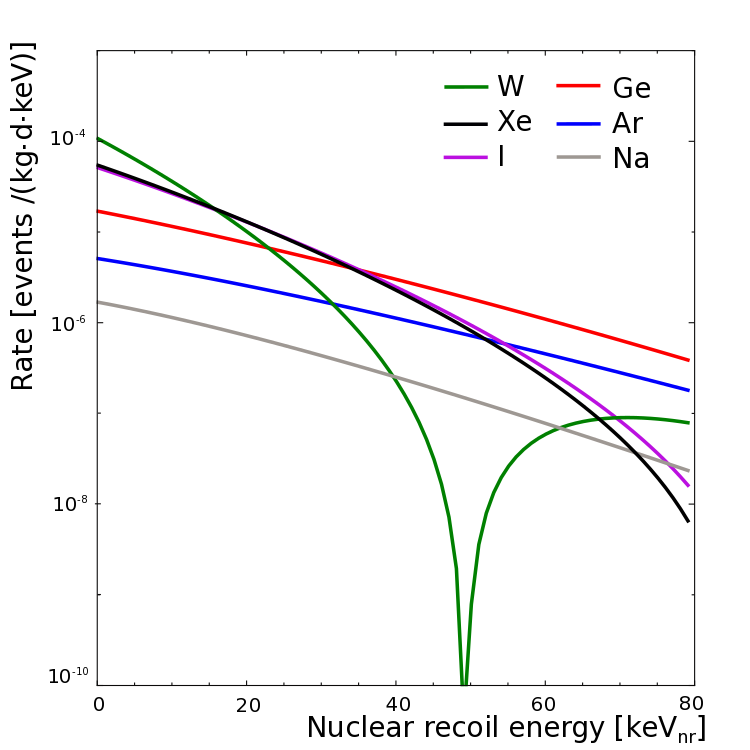
\includegraphics[width=0.4\textwidth]{figures/dm/rate_comp_v03} & 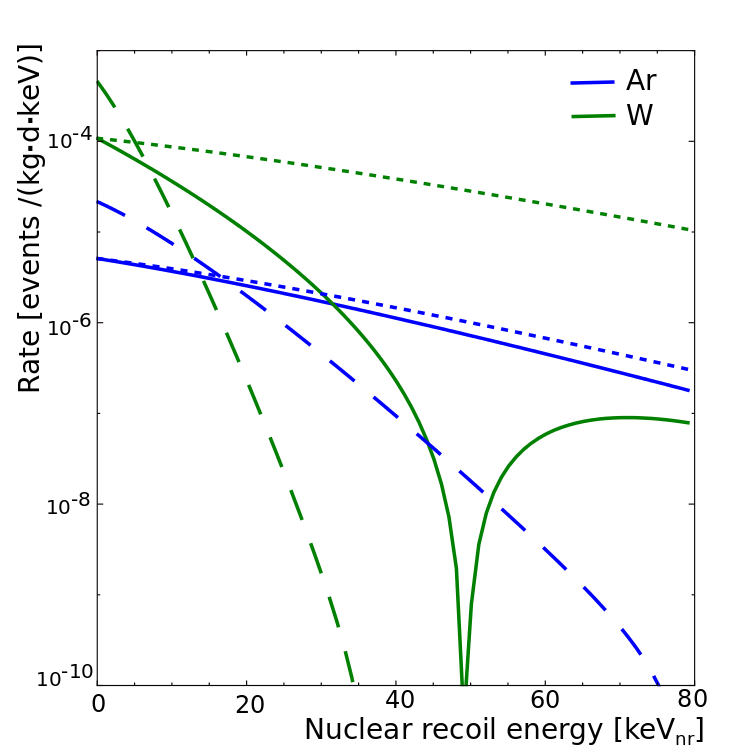
\includegraphics[width=0.4\textwidth]{figures/dm/rate_var_vs01} \\
    \end{tabular}
    \caption{(Left) WIMP differential interaction rate for a particle of mass $100\1{GeV/c^2}$ and cross-section $10^{-45}\1{cm^2}$ for a variety of different target materials. (Right) Reducing the WIMP mass to $25\1{GeV/c^2}$ yields the dashed lines, and neglecting the form factor yields the dotted lines. Figures from~\cite{Undagoitia:2015gya}.}~\label{fig:dm_rate}
\end{figure}

Reducing the mass of the dark matter particle increases the number density (as the energy density is fixed) and consequently the flux of particles through the detector, but as the particle velocity is constrained lower mass means lower energy, which in turn means less energy deposited in the detector. Likewise, increasing the dark matter mass reduces the flux but means the particles have higher energies.

\subsubsection{Annual modulation}

As the earth orbits around the sun, the sun in turn orbits the galactic center. In June, the velocities of the earth and sun are aligned, and in December they are antialigned. Thus, during June the flux of dark matter particles through a detector is slightly larger and in December is slightly less. Following~\cite{Freese:2012xd}, we express the energy spectrum as a Fourier series, of which the first two terms are
\begin{equation}\label{eq:modulation}
\frac{dR}{dE}(E,t) = S_0(E) + S_m(E)\cos (\omega t - \phi)
\end{equation}
where $S_0$ is the rate averaged over one year, $S_m$ the modulation amplitude (subject to $|S_m| \ll S_0$), $\omega = (2\pi)/(1~\n{year})$ the angular frequency, and $\phi$ the phase offset, set such that the rate has a maximum in June. Assuming that the detector operational stability is good for period of approximately one year or more, a modulation in the event rate can be measured and some potential dark matter interaction investigated~\cite{Aprile:2017yea,Abe:2018mxq}.

\paragraph{Conclusion} In this chapter we have investigated some of the evidence for the existence of dark matter, which constitutes much more of the universe than the protons and neutrons we are most familiar with. We discussed some detection strategies and results, and looked at some of the details of direct detection experiments, which will be the focus of this thesis.